\section{Casi d'uso}
\subsection{Attore}
Poiché per lo svolgimento del progetto non è necessario gestire permessi differenti per l'accesso alle funzionalità, l'attore che interagisce con il nostro software è unico, denominato "Utente".\\
\textbf{Utente:} soggetto che utilizza la web application, sfruttandone le funzionalità.
\subsection{UC1 - Visualizzazione lista dei dataset disponibili}
\begin{figure}[h!]
    \centering
    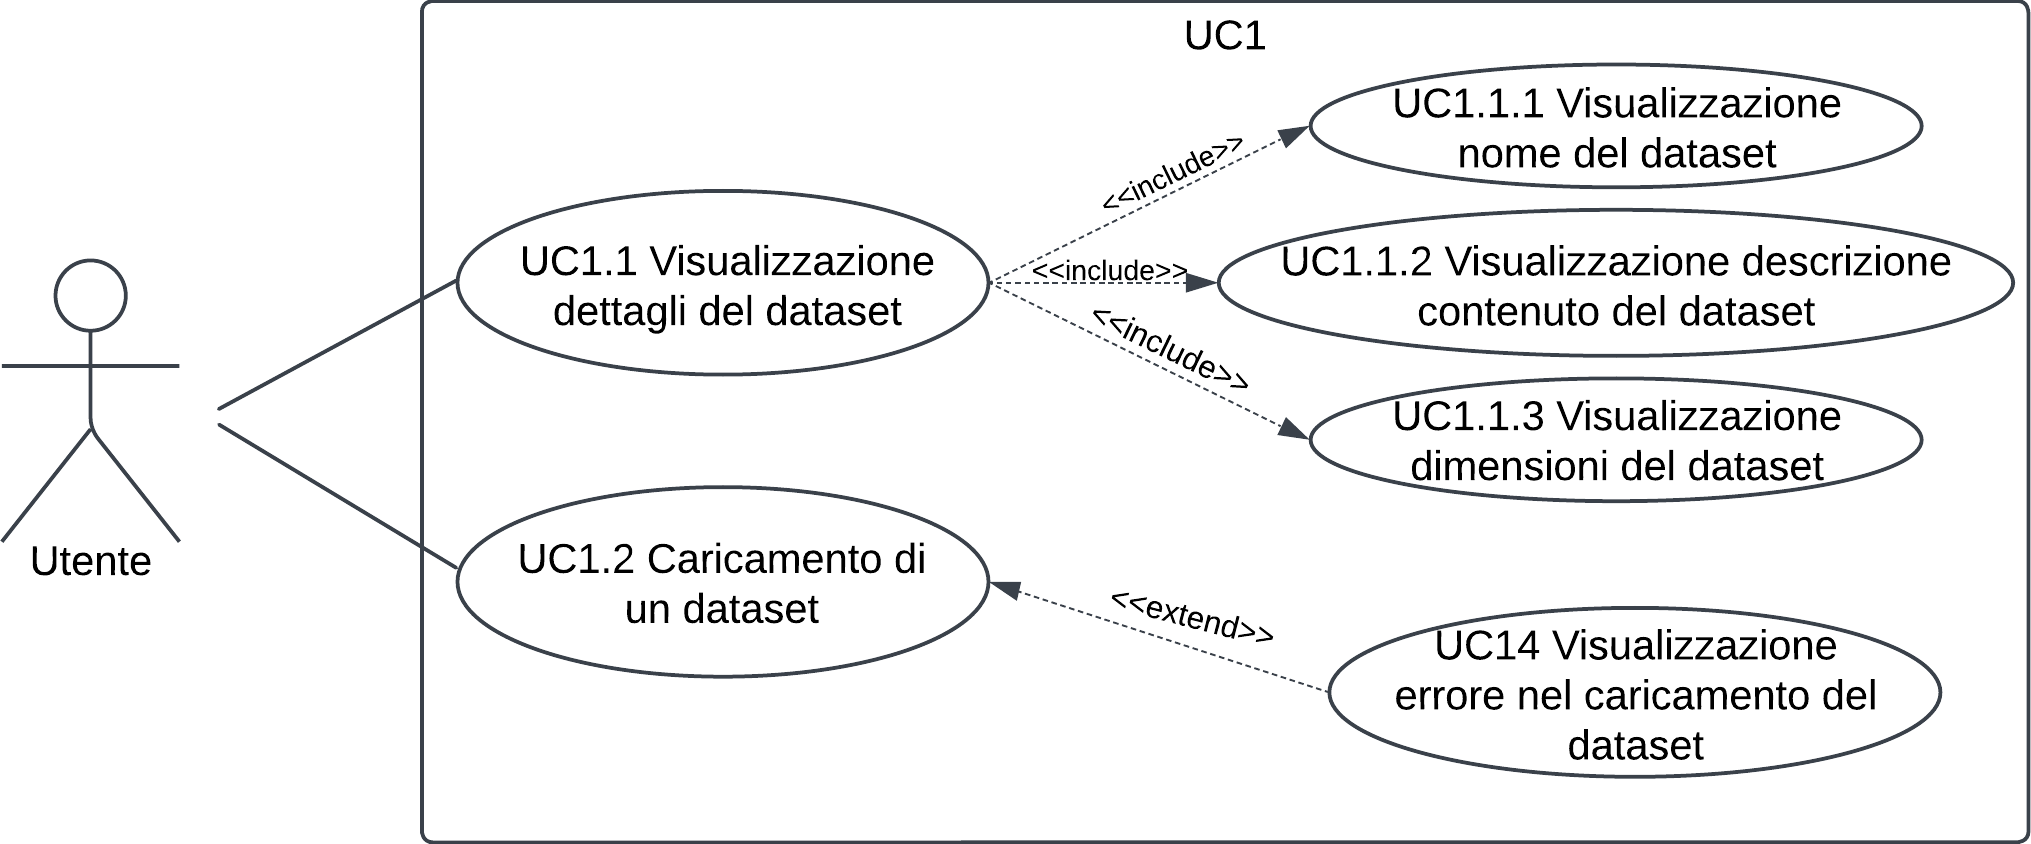
\includegraphics[scale=0.7]{template/images/UC1.png}
    \caption{UC1 - Visualizzazione lista dei dataset disponibili}
\end{figure}
\begin{itemize}
    \item \textbf{Attore:} utente;
    \item \textbf{Descrizione:} quando un utente interagisce con l'applicazione web,
    gli viene mostrato un elenco di dataset.\\ Da questa lista, può scegliere il dataset da rappresentare sotto forma di tabella e di grafico 3D.
    \item \textbf{Precondizioni:}
    \begin{itemize}
        \item L'utente ha accesso all'applicazione.
    \end{itemize}
    \item \textbf{Postcondizioni:}
    \begin{itemize}
        \item L'utente vede una lista dei dataset disponibili.
    \end{itemize}
    \item \textbf{Scenario:} 
    \begin{itemize}
        \item L'utente avvia il sistema;
        \item I dataset disponibili vengono presentati tramite un elenco;
        \item L'utente può navigare l'elenco e scegliere il dataset che gli interessa.
    \end{itemize}
\end{itemize}
\newpage
\subsubsection{UC1.1 - Visualizzazione dettagli del dataset}
\begin{itemize}
    \item \textbf{Attore:} utente;
    \item \textbf{Descrizione:} permette di visualizzare i dettagli del dataset selezionato;
    \item \textbf{Precondizioni:}
    \begin{itemize}
        \item Il sistema ha accesso ai dettagli tecnici e descrittivi del dataset.
    \end{itemize}
    \item \textbf{Postcondizioni:}
    \begin{itemize}
        \item Le informazioni sul dataset vengono mostrate all'utente.
    \end{itemize}
    \item \textbf{Scenario:}
    \begin{itemize}
        \item Il sistema mostra i dettagli dei dataset presenti nell'elenco.
    \end{itemize}
\end{itemize}
\paragraph{UC1.1.1 - Visualizzazione nome del dataset}
\begin{itemize}
    \item \textbf{Attore:} utente;
    \item \textbf{Descrizione:} l'utente può visualizzare il nome del dataset presente nell'elenco;
    \item \textbf{Precondizioni:}
    \begin{itemize}
        \item Il sistema ha accesso alle informazioni sul dataset.
    \end{itemize}
    \item \textbf{Postcondizioni:}
    \begin{itemize}
        \item Il nome del dataset viene mostrato all'utente.
    \end{itemize}
    \item \textbf{Scenario:}
    \begin{itemize}
        \item Il sistema mostra il nome del dataset.
    \end{itemize}
\end{itemize}
\paragraph{UC1.1.2 - Visualizzazione della descrizione contenuto del dataset}
\begin{itemize}
    \item \textbf{Attore:} utente;
    \item \textbf{Descrizione:} l'utente può visualizzare una descrizione del contenuto del dataset;
    \item \textbf{Precondizioni:}
    \begin{itemize}
        \item Il sistema ha accesso alle informazioni relative al contenuto del dataset.
    \end{itemize}
    \item \textbf{Postcondizioni:}
    \begin{itemize}
        \item La descrizione del contenuto del dataset viene mostrata all'utente.
    \end{itemize}
    \item \textbf{Scenario:}
    \begin{itemize}
        \item Il sistema mostra una descrizione del contenuto del dataset.
    \end{itemize}
\end{itemize}
\paragraph{UC1.1.3 - Visualizzazione dimensioni tabella}
\begin{itemize}
    \item \textbf{Attore:} utente;
    \item \textbf{Descrizione:} l'utente può visualizzare le dimensioni della tabella relativa ai dati contenuti nel dataset;
    \item \textbf{Precondizioni:}
    \begin{itemize}
        \item Il sistema ha accesso alle informazioni relative alla dimensione del dataset.
    \end{itemize}
    \item \textbf{Postcondizioni:}
    \begin{itemize}
        \item Le dimensioni della tabella relativa ai dati contenuti nel dataset vengono mostrate all'utente.
    \end{itemize}
    \item \textbf{Scenario:}
    \begin{itemize}
        \item Il sistema mostra le dimensioni della tabella relativa ai dati contenuti nel dataset.
    \end{itemize}
\end{itemize}

\subsubsection{UC1.2 - Caricamento di un dataset dall'elenco di quelli disponibili}
\begin{itemize}
    \item \textbf{Attore:} utente;
    \item \textbf{Descrizione:} consente di caricare il dataset selezionato nell'ambiente 3D dell'applicazione;
    \item \textbf{Precondizioni:}
    \begin{itemize}
        \item L'elenco dei dataset disponibili è stato caricato correttamente;
    \end{itemize}
    \item \textbf{Postcondizioni:}
    \begin{itemize}
        \item Il dataset selezionato viene caricato nel sistema.
    \end{itemize}
    \item \textbf{Scenario:}
    \begin{itemize}
        \item L'utente seleziona un dataset dall'elenco disponibile;
        \item Il sistema prepara i dati per la visualizzazione in forma tabellare e in grafico 3D.
    \end{itemize}
\end{itemize}
\newpage
\subsection{UC2 - Visualizzazione dati in forma tabellare}
\begin{figure}[h!]
    \centering
    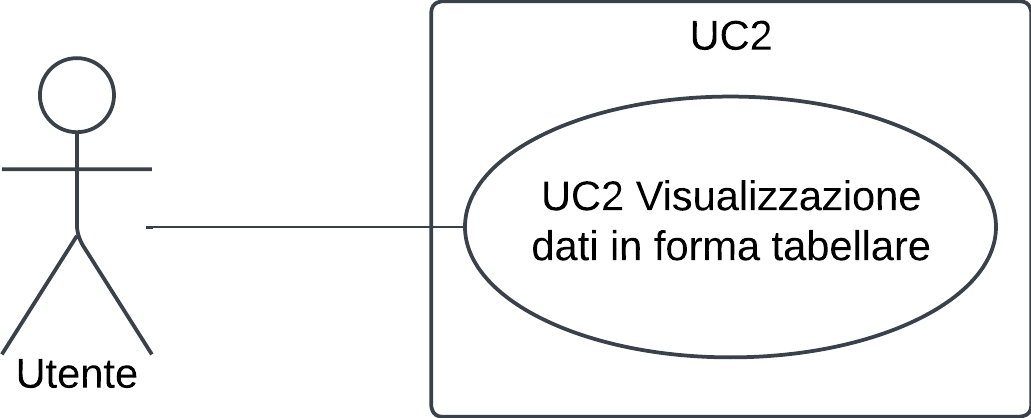
\includegraphics[scale=0.7]{template/images/UC2.png}
    \caption{UC2 - Visualizzazione dati in forma tabellare}
\end{figure}
\begin{itemize}
    \item \textbf{Attore:} utente;
    \item \textbf{Descrizione:} consente di visualizzare il dataset caricato sotto forma di tabella;
    \item \textbf{Precondizioni:}
    \begin{itemize}
        \item Il dataset selezionato è stato caricato correttamente.
    \end{itemize}
    \item \textbf{Postcondizioni:}
    \begin{itemize}
        \item I dati sono mostrati in forma tabellare.
    \end{itemize}
    \item \textbf{Scenario:}
    \begin{itemize}
        \item Il dataset selezionato viene caricato correttamente;
        \item L'applicazione elabora i dati e vengono mostrati in forma tabellare.
    \end{itemize}
\end{itemize}
\subsection{UC3 - Visualizzazione dati in forma di grafico a istogramma 3D verticale}
\begin{figure}[h!]
    \centering
    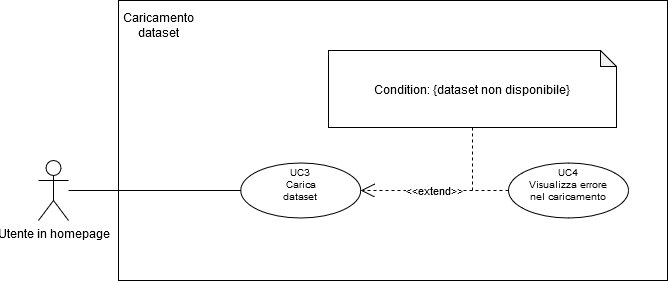
\includegraphics[scale=0.7]{template/images/UC3.png}
    \caption{UC3 - Visualizzazione dati in forma di grafico a istogramma 3D verticale}
\end{figure}
\begin{itemize}
    \item \textbf{Attore:} utente;
    \item \textbf{Descrizione:} consente di visualizzare il dataset caricato sotto forma di grafico a istogramma 3D verticale;
    \item \textbf{Precondizioni:}
    \begin{itemize}
        \item Il dataset selezionato è stato caricato correttamente.
    \end{itemize}
    \item \textbf{Postcondizioni:}
    \begin{itemize}
        \item I dati sono mostrati in forma di grafico a istogramma 3D verticale.
    \end{itemize}
    \item \textbf{Scenario:}
    \begin{itemize}
        \item Il dataset viene caricato correttamente;
        \item L'applicazione elabora i dati e viene creato un grafico a istogramma 3D verticale;
        \item L'interfaccia visualizza il grafico 3D verticale in una vista interattiva, consentendo all'utente di analizzare i dati.
    \end{itemize}
\end{itemize}
\subsection{UC4 - Visualizzazione assi}
\begin{itemize}
    \item \textbf{Attore:} utente;
    \item \textbf{Descrizione:} consente di visualizzare dettagliatamente gli assi X, Y e Z del grafico;
    \item \textbf{Precondizioni:} 
    \begin{itemize}
        \item Il grafico 3D è stato generato correttamente;
        \item Gli assi sono correttamente configurati nel sistema.
    \end{itemize}
    \item \textbf{Postcondizioni:}
    \begin{itemize}
        \item Gli assi X, Y e Z sono visibili e ben etichettati.
    \end{itemize}
    \item \textbf{Scenario:}
    \begin{itemize}
        \item L'utente visualizza il grafico 3D;
        \item L'utente visualizza gli assi X,Y e Z.
    \end{itemize}

\end{itemize}
\subsubsection{UC4.1 - Visualizzazione asse X}
\begin{itemize}
    \item \textbf{Attore:} utente;
    \item \textbf{Descrizione:} consente di visualizzare dettagliatamente l'asse X;
    \item \textbf{Precondizioni:} 
    \begin{itemize}
        \item L'asse X è configurato nel grafico.
    \end{itemize}
    \item \textbf{Postcondizioni:} 
    \begin{itemize}
        \item L'asse X è visibile e mostra i valori appropriati.
    \end{itemize}
    \item \textbf{Scenario:} 
    \begin{itemize}
        \item L'utente visualizza il grafico 3D;
        \item L'utente visualizza l'asse X con i valori appropriati.
    \end{itemize}
\end{itemize}
\subsubsection{UC4.2 - Visualizzazione asse Y}
\begin{itemize}
    \item \textbf{Attore:} utente;
    \item \textbf{Descrizione:} consente di visualizzare dettagliatamente l'asse Y;
    \item \textbf{Precondizioni:} 
    \begin{itemize}
        \item L'asse Y è configurato nel grafico.
    \end{itemize}
    \item \textbf{Postcondizioni:} 
    \begin{itemize}
        \item L'asse Y è visibile e mostra i valori appropriati.
    \end{itemize}
    \item \textbf{Scenario:} 
    \begin{itemize}
        \item L'utente visualizza il grafico 3D;
        \item L'utente visualizza l'asse Y con i valori appropriati.
    \end{itemize}
\end{itemize}
\subsubsection{UC4.3 - Visualizzazione asse Z}
\begin{itemize}
    \item \textbf{Attore:} utente;
    \item \textbf{Descrizione:} consente di visualizzare dettagliatamente l'asse Z;
    \item \textbf{Precondizioni:} 
    \begin{itemize}
        \item L'asse Z è configurato nel grafico.
    \end{itemize}
    \item \textbf{Postcondizioni:} 
    \begin{itemize}
        \item L'asse Z è visibile e mostra i valori appropriati.
    \end{itemize}
    \item \textbf{Scenario:} 
    \begin{itemize}
        \item L'utente visualizza il grafico 3D;
        \item L'utente visualizza l'asse Z con i valori appropriati.
    \end{itemize}
\end{itemize}
\subsection{UC5 - Visualizzazione legenda}
\begin{itemize}
    \item \textbf{Attore:} utente;
    \item \textbf{Descrizione:} consente di visualizzare una legenda con dettagli e informazioni sul grafico;
    \item \textbf{Precondizioni:} 
    \begin{itemize}
        \item Il grafico 3D è stato generato correttamente;
        \item Il sistema dispone delle informazioni necessarie per creare una legenda.
    \end{itemize}
    \item \textbf{Postcondizioni:}
    \begin{itemize}
        \item La legenda è visibile e fornisce informazioni dettagliate che aiutano l'utente a comprendere i dati rappresentati.
    \end{itemize}
    \item \textbf{Scenario:} 
    \begin{itemize}
        \item Il grafico viene generato correttamente;
        \item La legenda relativa al grafico è visibile.
    \end{itemize}
\end{itemize}
\subsection{UC6 - Pan}
\begin{figure}[h!]
    \centering
    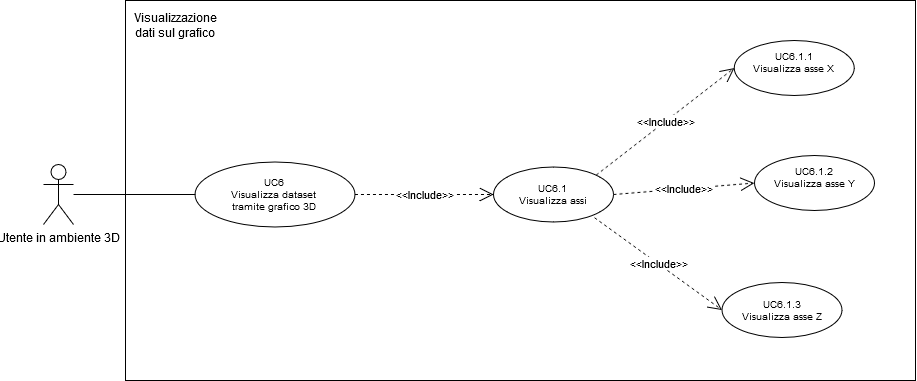
\includegraphics[scale=0.7]{template/images/UC6.png}
    \caption{UC6 - PAN}
\end{figure}
\begin{itemize}
    \item \textbf{Attore:} utente;
    \item \textbf{Descrizione:} l'utente sposta la visualizzazione del grafico 3D lungo il piano XY senza modificare l'orientamento della camera;
    \item \textbf{Precondizioni:}
    \begin{itemize}
        \item L'utente sta visualizzando il grafico 3D;
        \item Il sistema ha abilitato la funzionalità di interazione pan.
    \end{itemize}
    \item \textbf{Postcondizioni}:
    \begin{itemize}
        \item La vista della scena 3D è stata spostata nella direzione indicata dall'utente.
    \end{itemize}
    \item \textbf{Scenario:}
    \begin{itemize}
        \item L'utente visualizza il grafico 3D nell'interfaccia;
        \item L'utente interagisce con il grafico utilizzando il mouse (trascinamento);
        \item Il sistema interpreta il comando di spostamento e aggiorna la posizione del grafico lungo il piano XY;
        \item La nuova vista viene aggiornata in tempo reale e mostrata all'utente.
    \end{itemize}
\end{itemize}
\subsection{UC7 - Rotazione camera}
\begin{figure}[h!]
    \centering
    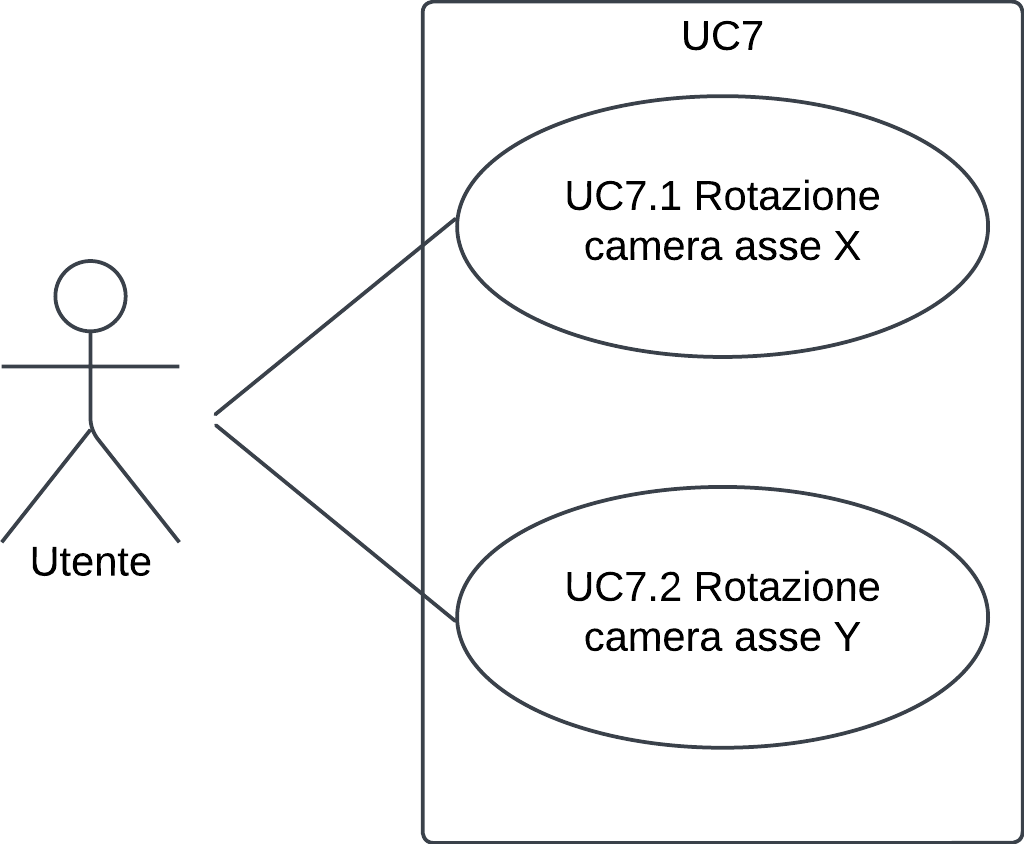
\includegraphics[scale=0.7]{template/images/UC7_7.1_7.2.png}
    \caption{UC7 - Rotazione camera}
\end{figure}
\begin{itemize}
    \item \textbf{Attore:} utente;
    \item \textbf{Descrizione:} l'utente ruota la visualizzazione del grafico 3D modificando l'orientamento della camera lungo uno o più assi. La rotazione consente di analizzare il grafico da diverse angolazioni;
    \item \textbf{Precondizioni:} 
    \begin{itemize}
        \item L'utente sta visualizzando il grafico 3D nell'interfaccia;
        \item Il sistema ha abilitato le funzionalità di interazione con la camera.
    \end{itemize}
    \item \textbf{Postcondizioni:} 
    \begin{itemize}
        \item La visualizzazione del grafico è stata aggiornata in base alla rotazione effettuata dall'utente.
    \end{itemize}
    \item \textbf{Scenario:} 
    \begin{itemize}
        \item L'utente interagisce con il grafico 3D usando i comandi per ruotare la visualizzazione. Il sistema aggiorna in tempo reale l'orientamento della camera, mostrando il grafico da una nuova angolazione.
    \end{itemize}
    
\end{itemize}
\subsubsection{UC7.1 - Rotazione camera asse X}
\begin{itemize}
    \item \textbf{Attore:} utente;
    \item \textbf{Descrizione:} l'utente ruota la visualizzazione del grafico 3D attorno all'asse X, modificando l'altezza della prospettiva.
    \item \textbf{Precondizioni:} 
    \begin{itemize}
        \item L'utente sta visualizzando il grafico 3D nell'interfaccia;
        \item Il sistema ha abilitato le funzionalità di interazione con la camera.
    \end{itemize}
    \item \textbf{Postcondizioni:} 
    \begin{itemize}
        \item La camera è stata ruotata attorno all'asse X, aggiornando la vista in tempo reale.
    \end{itemize}
    \item \textbf{Scenario:}
    \begin{itemize}
        \item L'utente usa comandi per spostare la vista verso l'alto o verso il basso. Il sistema ruota la camera attorno all'asse X, consentendo di osservare il grafico da un'angolazione più alta o più bassa.
    \end{itemize}
    
\end{itemize}
\subsubsection{UC7.2 - Rotazione camera asse Y}
\begin{itemize}
    \item \textbf{Attore:} utente;
    \item \textbf{Descrizione:} l'utente ruota la visualizzazione del grafico 3D attorno all'asse Y, modificando l'orientamento laterale della prospettiva;
    \item \textbf{Precondizioni:} 
    \begin{itemize}
        \item L'utente sta visualizzando il grafico 3D nell'interfaccia;
        \item Il sistema ha abilitato le funzionalità di interazione con la camera.
    \end{itemize}
    \item \textbf{Postcondizioni:} 
    \begin{itemize}
        \item La camera è stata ruotata attorno all'asse Y, aggiornando la vista in tempo reale.
    \end{itemize}
    \item \textbf{Scenario:} 
    \begin{itemize}
        \item L'utente usa comandi per spostare la vista verso destra o sinistra. Il sistema ruota la camera attorno all'asse Y, consentendo di osservare il grafico da angolazioni diverse lateralmente.
    \end{itemize}
\end{itemize}


